
\subsection{Main Objectives}
Considering the challenges we mentioned on the previous section. We came up  to the conclusion that in order to have a clear output we have to come up with a new approach while keeping the main points and ideas that are presented in the main article. So lets review what are the main values delivered in the article: 
\begin{itemize}
    \item Use letter-n-grams in order to build a feature set to predict the sound of a word
    \item Find a mapping from letter-n-gram feature space into  a dense embedded space. In such space our assumption is that words with similar sound will stay close to each other
    \item Ability to map words that are not in speech corpus to embedding space    
\end{itemize}

If we target all of above objectives, with slightly different approach then we can say we have delivered  the project. The point is that this is the new potential for publication as we are incorporating a novel approach. 

\subsection{Overcoming Challenges}
The hardest challenge to address in the project was to access  the end-to-end speech recognition neural network that is described in the article. Two main challenges there, no data set and also the processing time for such big network is huge. So I made an executive decision to find alternative pre-trained models to enable us to focus on the embedding part of the task. 

After looking at available systems I concluded to use Deep Speech system. 

\subsubsection{Deep Speech}
Project DeepSpeech is an open source Speech-To-Text engine, using a model trained by machine learning techniques, based on \cite{DBLP:journals/corr/HannunCCCDEPSSCN14}. Project DeepSpeech uses Google's TensorFlow project to make the implementation easier.

This network is a bidirectional RNN. The core of the system is a recurrent neural network (RNN) trained to ingest speech spectrograms and generate English text transcriptions. The goal of the  RNN is to convert an input sequence $x$ into a sequence of character probabilities for the transcription $y$. The RNN model is composed of 5 layers of hidden units.  Deep Speech has been  implemented by Mozilla team as open package. It is available on Github.   

\begin{figure}[hbt!]
    \centering
    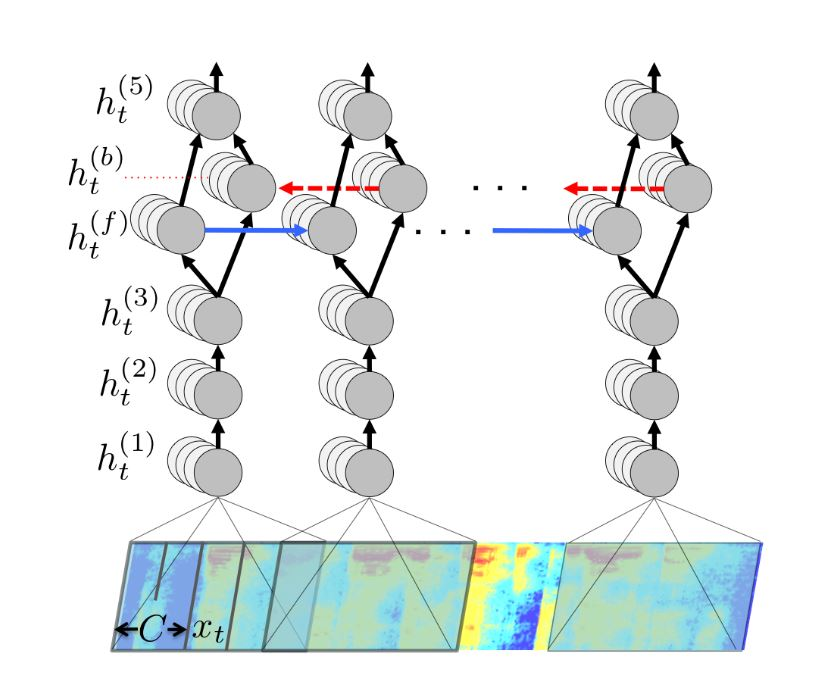
\includegraphics{Images/rnn.jpg}    
    \caption{RNN Architecture}
    \label{rnn_arch}
\end{figure}


We are going to use this model to create the embedding layer of the project.  This network is producing a series of probabilities of the alphabet. This includes space character and apostrophe. we are going to process the words and concatenate the probability vectors of words as the  embedded version of the word that is spoken. 

\begin{figure}[hbt!]
    \centering
    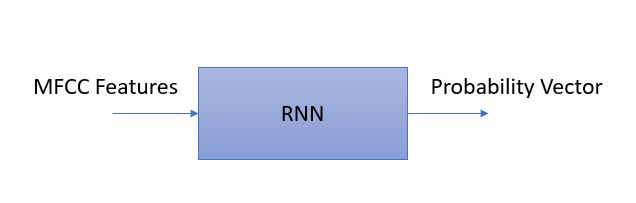
\includegraphics{Images/simple_model.jpg}    
    \caption{The simplistic view of the RNN}
    \label{simple_view}
\end{figure}

For each word then the concatenation of the probability vectors is going to make the embedding vector. Based on the size of the word in the input file we decided to make $N=10$ as the number of concatenated vectors. So for each word $N$ alphabet probability vectors are concatenated. If the length of the word was less than $N$ then empty padding vectors were added to it to make all inputs having the same shape.  

\subsubsection{Dataset}
I decided to use Librispeech dataset. This dataset contains over 1000 hours of speech corpus. It is organized in to multiple collections: 
\begin{itemize}
    \item Dev Clean 
    \item Test Clean 
    \item test Clean 
    \item Train Clean 100
    \item Train Clean 360
    \item Train Clean 500
\end{itemize}

In this project we only used the Dev clean dataset. This data set contains 2800 audio files that  each file is one or more sentence. Each file is transcripted. But transcription is in sentence level so the file is not tagged on word level. 

Audio files were in FLAC format. So for being used by our library, we had to convert them into wav in addition to that the folder structure was a bit deep make it a little bit hard to work with. For this reason I write a conversion code to convert the file into WAV format and also put the information into one master excel-sheet for easier processing. 

\subsubsection{Creating Word Level Data}
As we said the transcriptions of the files are on sentence level. From the other hand the RNN is producing the probability vectors on letter level.  For purpose of this project we needed the  probability vectors on word level. So we needed to write a code to give us the data we want. 

A code was written to use RNN pretrained model available on Mozilla DeepSpeech project to process all audio files and produce the character level probability vectors. Then using the probability vector to generate the raw transcription of the files. 
As we only had access to sentence level transcription of the files to build the dataset we had to match between them. As the output of the RNN had lots of errors matching was challenging. After processing file, it seems that using Longest Common Sequence method is going to give us a good result. So LCS method was implemented to break down the word level data. 
After processing the files the data set resulted in 57000 word level data instances which were stored in CSV file format for further use. 

\subsection{Preparing the Word Letter-N-Grams}
Lat piece of the input puzzle was the letter-n-gram input vectors. A code was written to create the index file for letter-n-grams to be used for both training and testing. One of the hyper parameters here was the maximum n to build n-grams. In this experiment we used  $N = 4$ which resulted in 4737 features. This became the dimension of input for the embedding neural network. 
\subsubsection{Embedding Network}

After data was prepared, we are ready to implement our embedding neural network. The embedding neural network was implemented usnig Tensorflow and Keras. The architecture is an auto-encoder with one hidden layer. The actiovation function of the thin hidden layer is RelU function. For test purpose we set the size of hidden layer unit to be $h = 300$.  The output layer is actually a set of independent output Softmax layers for each character. The network trained with \textit{AdamOptimizer} with 20 epochs. 



